\documentclass[border=3pt]{standalone}
\usepackage[T1]{fontenc}
\usepackage[utf8]{inputenc}
\usepackage{lmodern}
\usepackage{amsmath,amssymb}
\usepackage{xcolor}
\usepackage{tikz}
\usepackage{fontawesome5}
\usepackage{ragged2e}
\usetikzlibrary{shapes,shapes.geometric,shapes.misc,arrows.meta,positioning,
                calc,fit,backgrounds,decorations.pathreplacing,
                decorations.markings,patterns,chains}
\usetikzlibrary{decorations.pathreplacing,decorations.markings}
\definecolor{primary}{HTML}{1A5276}
\definecolor{secondary}{HTML}{2E86C1}
\definecolor{accent}{HTML}{E74C3C}
\definecolor{lightbg}{HTML}{EBF5FB}
\definecolor{defbg}{HTML}{FDF2E9}
\definecolor{greenhl}{HTML}{27AE60}
\definecolor{purplehl}{HTML}{8E44AD}
\definecolor{goldhl}{HTML}{B7950B}
\definecolor{tealhl}{HTML}{117A65}
\definecolor{codebg}{HTML}{F4F6F7}
\definecolor{neutral}{HTML}{707B7C}
\definecolor{dom1}{HTML}{1F618D}
\definecolor{dom2}{HTML}{117864}
\definecolor{dom3}{HTML}{6C3483}
\definecolor{dom4}{HTML}{922B21}
\definecolor{dom5}{HTML}{B7950B}
% --- carried over from ccna.sty so figures match the book exactly
\tikzset{
  dev/.style={rounded corners=3pt, draw=#1, fill=#1!8, text=#1!45!black,
              line width=0.9pt, minimum width=1.45cm, minimum height=1.05cm,
              align=center, font=\scriptsize\bfseries, inner sep=2pt},
  wirestyle/.style={line width=0.9pt, neutral!75},
  xconn/.style={line width=0.9pt, neutral!75, dash pattern=on 2.5pt off 2pt},
}

\newcommand{\Rtr}[3]{\node[dev=dom3] (#1) at #2 {\faIcon{route}\\#3};}
\newcommand{\Sw}[3]{\node[dev=dom2] (#1) at #2 {\faIcon{sitemap}\\#3};}
\newcommand{\Msw}[3]{\node[dev=dom3] (#1) at #2 {\faIcon{layer-group}\\#3};}
\newcommand{\Host}[3]{\node[dev=neutral] (#1) at #2 {\faIcon{desktop}\\#3};}
\newcommand{\Lap}[3]{\node[dev=neutral] (#1) at #2 {\faIcon{laptop}\\#3};}
\newcommand{\Srv}[3]{\node[dev=dom1] (#1) at #2 {\faIcon{server}\\#3};}
\newcommand{\Ap}[3]{\node[dev=dom5] (#1) at #2 {\faIcon{wifi}\\#3};}
\newcommand{\Wlc}[3]{\node[dev=dom5] (#1) at #2 {\faIcon{broadcast-tower}\\#3};}
\newcommand{\Fw}[3]{\node[dev=dom4] (#1) at #2 {\faIcon{shield-alt}\\#3};}
\newcommand{\Cld}[3]{\node[dev=neutral] (#1) at #2 {\faIcon{cloud}\\#3};}
\newcommand{\Phone}[3]{\node[dev=dom5] (#1) at #2 {\faIcon{phone-alt}\\#3};}
\newcommand{\Prn}[3]{\node[dev=neutral] (#1) at #2 {\faIcon{print}\\#3};}

% A link. The optional argument takes tikz options (e.g. xconn for a
% trunk drawn dashed); the fourth argument labels the link.
\newcommand{\wire}[4][wirestyle]{%
  \draw[#1] (#2) -- node[font=\tiny, text=neutral!85!black, fill=white,
                          inner sep=1.2pt, midway] {#4} (#3);}
\newcommand{\plainwire}[3][wirestyle]{\draw[#1] (#2) -- (#3);}


\newenvironment{topology}[1][]
  {\begin{center}\begin{tikzpicture}[font=\scriptsize,#1]}
  {\end{tikzpicture}\end{center}}


\newcommand{\cmd}[1]{\texttt{\small #1}}
\newcommand{\term}[1]{\textbf{\textcolor{primary}{#1}}}
\newcommand{\chref}[1]{Chapter~\ref{ch:#1}}
\newcommand{\ccnafitw}[1]{#1}
\providecommand{\thefigure}{}
% --- progressive builds
\newcount\buildlevel \buildlevel=99
% \stepvis{n}{..} appears from level n onward; \steponly{n}{..} at
% level n alone, which is how a caption is swapped rather than
% accumulated as the build advances. \stepdim{n}{..} is the
% complement of \stepvis: it shows only BEFORE level n, so a
% pair of them draws an element faint and then solid. That keeps
% the canvas full from step 1, which matters for a figure whose
% shape is itself the lesson -- a five-rung ladder revealed one
% rung at a time leaves a void where the method should be.
\newcommand{\stepvis}[2]{\ifnum#1>\buildlevel\relax\else#2\fi}
\newcommand{\steponly}[2]{\ifnum#1=\buildlevel #2\fi}
\newcommand{\stepdim}[2]{\ifnum#1>\buildlevel #2\fi}
% Slide text does not hyphenate. A projected caption broken as
% ``uni-cast'' costs the reader a beat that print can afford and a
% lecture cannot, and the ragged edge it avoids is invisible at
% four metres anyway.
\hyphenpenalty=10000 \exhyphenpenalty=10000
\begin{document}
\buildlevel=1
% Slide build of Figure 21.1 -- resolution one hop at a time.
%
% The whole point of the figure is that step 1 is recursive and steps 2-4 are
% iterative: the host asks once and waits, the resolver does the walking. Drawn
% all at once, that distinction is a thing the lecturer asserts. Built up, the
% room watches the host go quiet after step 1 while the resolver runs around,
% and the assertion is unnecessary.
%
% Step 5 adds the cache, because "and it remembers for the TTL" is the answer
% to "why is it fast the second time" and to half of chapter 21's Break & Fix.
\begin{tikzpicture}[font=\scriptsize]
  % Fixed canvas: the widest step must not resize the picture, or Morph
  % translates the whole diagram instead of fading the new arrow in.
  \path (-2.1,-4.3) rectangle (11.9,2.7);

  \tikzset{
    bx/.style={rounded corners=3pt, draw=#1, fill=#1!8, text=#1!45!black,
               line width=0.9pt, text width=2.5cm, align=center,
               minimum height=1.15cm, font=\scriptsize\bfseries},
    q/.style={-{Stealth[length=2.2mm]}, line width=0.9pt, dom4!75},
    a/.style={-{Stealth[length=2.2mm]}, line width=0.9pt, dom1!70,
              dash pattern=on 2.5pt off 2pt},
    stepcap/.style={font=\bfseries, anchor=north west, text width=12.6cm,
                    align=left}}

  \node[bx=neutral] (h)  at (0,0)     {\faIcon{desktop}\\[1pt]Host\\
      \footnotesize\mdseries stub resolver};
  \node[bx=dom1]    (rec) at (4.9,0)  {\faIcon{server}\\[1pt]Recursive\\
      \footnotesize\mdseries resolver, caches};
  \node[bx=dom4]    (rt)  at (9.7,1.5){\faIcon{globe}\\[1pt]Root\\
      \footnotesize\mdseries ``ask .edu''};
  \node[bx=dom4]    (tld) at (9.7,0)  {\faIcon{globe}\\[1pt]TLD .edu\\
      \footnotesize\mdseries ``ask them''};
  \node[bx=dom4]    (au)  at (9.7,-1.5){\faIcon{database}\\[1pt]Authoritative\\
      \footnotesize\mdseries holds the zone};

  % Query below the line, answer above the arc that bends over it. With both
  % on the inside they printed on top of each other in the gap between the
  % nodes -- which the book did too, and is now fixed in both.
  \stepvis{1}{\draw[q] (h) -- node[font=\tiny, below, midway,
      text=dom4!45!black] {1. recursive query} (rec);}
  \stepvis{2}{\draw[q] (rec) -- node[font=\tiny, above=1pt, pos=0.6] {2} (rt);}
  \stepvis{3}{\draw[q] (rec) -- node[font=\tiny, above=1pt, pos=0.6] {3} (tld);}
  \stepvis{4}{\draw[q] (rec) -- node[font=\tiny, above=1pt, pos=0.6] {4} (au);}
  \stepvis{5}{\draw[a] (rec) to[bend right=22]
      node[font=\tiny, above, midway, text=dom1!45!black]
      {5. answer, with a TTL} (h);}

  % The host is doing nothing at all during 2-4. Saying so on the diagram
  % is worth more than saying it aloud -- and it has to come off again at
  % step 5, when the host is no longer waiting for anything.
  \stepvis{2}{\stepdim{5}{\node[font=\tiny\itshape, text=neutral!70!black,
      anchor=north] at (0,-1.0) {still waiting};}}

  \stepvis{5}{%
    \node[draw=dom1!55, fill=dom1!8, rounded corners=3pt, line width=0.8pt,
          font=\tiny\ttfamily, align=left, inner sep=5pt, anchor=north west]
        at (3.4,-1.9)
        {\textcolor{dom1!45!black}{cache}\\ www.example.edu\\ TTL 3600};}

  \steponly{1}{\node[stepcap, text=dom4!45!black] at (-2.0,-3.0)
      {One question, then the host waits. This arrow is the only recursive
       one in the picture.};}
  \steponly{2}{\node[stepcap, text=dom4!45!black] at (-2.0,-3.0)
      {The root does not know the answer --- it knows who runs .edu.};}
  \steponly{3}{\node[stepcap, text=dom4!45!black] at (-2.0,-3.0)
      {Nor does the TLD. Each referral is one step down the name, right
       to left.};}
  \steponly{4}{\node[stepcap, text=dom4!45!black] at (-2.0,-3.0)
      {The authoritative server holds the zone, so this one answers.};}
  \steponly{5}{\node[stepcap, text=dom1!45!black] at (-2.0,-3.0)
      {The host gets one answer and never learns any of that happened ---
       and the resolver keeps it for the TTL, so the next host skips
       steps 2 to 4.};}
\end{tikzpicture}

\end{document}
